\documentclass[letterpaper, 10 pt, conference]{formatting/ieeeconf}
\IEEEoverridecommandlockouts                              % This command is only needed if 
                                                            % you want to use the \thanks command
\overrideIEEEmargins                                      % Needed to meet printer requirements.
\pdfminorversion=4			% ICRA standard
\let\labelindent\relax
\usepackage{amsfonts}       % An extended set of fonts for use in mathematics
\let\proof\relax
\let\endproof\relax
\usepackage{amsthm}
\usepackage{mathtools}      % Loads amsmath
\usepackage{amssymb}        % provides AMS fonts and symbols ex. \mathbb{...}
\usepackage{filecontents}
\usepackage{graphicx}       % enhanced support for graphics
\usepackage{marginnote}     % Add notes
\usepackage{marvosym}       % mvat
\usepackage{overpic}        % Add text on figures
\usepackage{tabularx}
\usepackage{cite}
\usepackage{color}
\usepackage[linesnumbered,algoruled,boxed,lined]{algorithm2e}
\usepackage[normalem]{ulem}
\usepackage{epstopdf}
\usepackage{graphicx}

\usepackage{epstopdf}
\usepackage{enumitem}
\usepackage[normalem]{ulem}
\usepackage{lipsum}
\usepackage{comment}

\usepackage{diagbox}
\usepackage{multirow}
\usepackage{caption}
\usepackage{subcaption}
\usepackage{CJKutf8}
\usepackage[dvipsnames]{xcolor}

%%%%%%%%%%%%%%%%%%%%%%%%%%%%%%%%%%%%%%%%%%%%%%%%%%%%%%%%%%%%%%%%%%%%%%%%
%%%%% Side comments   %%%%%%%%%%%%%%%%%%%%%%%%%%%%%%%%%%%%%%%%%%%%%%%%%%
%%%%%%%%%%%%%%%%%%%%%%%%%%%%%%%%%%%%%%%%%%%%%%%%%%%%%%%%%%%%%%%%%%%%%%%%
\newif\ifdraft
\draftfalse

\newif\ifoc % Single column?
\ocfalse

\usepackage[textsize=footnotesize]{todonotes}
\ifdraft
\usepackage[paperheight=11in,paperwidth=9.5in,
			left=1.25in,right=1.25in,
			top=0.75in,bottom=0.75in,
			heightrounded,marginparwidth=1.2in,
			marginparsep=0.05in]{geometry}
\usepackage{xcolor}
\usepackage{xargs} 
\newcommandx{\nt}[2][1=]{\todo[linecolor=red,
			backgroundcolor=red!10,bordercolor=red,#1]{#2}}
\newcommandx{\jy}[2][1=]{\todo[linecolor=green,
			backgroundcolor=green!10,bordercolor=green,#1]{JY: #2}}
\newcommandx{\sw}[2][1=]{\todo[linecolor=blue,
			backgroundcolor=blue!10,bordercolor=blue,#1]{SW: #2}}
\else
\newcommand{\nt}[1]{{}}
\newcommand{\jy}[1]{{}}
\newcommand{\sw}[1]{{}}
\fi

%%%%%%%%%%%%%%%%%%%%%%%%%%%%%%%%%%%%%%%%%%%%%%%%%%%%%%%%%%%%%%%%
% Spacing related commands.
%%%%%%%%%%%%%%%%%%%%%%%%%%%%%%%%%%%%%%%%%%%%%%%%%%%%%%%%%%%%%%%%
\newif\iftwocolumn
\twocolumntrue

%%%%%%%%%%%%%%%%%%%%%%%%%%%%%%%%%%%%%%%%%%%%%%%%%%%%%%%%%%%%%%%%
% Spacing related commands.
%%%%%%%%%%%%%%%%%%%%%%%%%%%%%%%%%%%%%%%%%%%%%%%%%%%%%%%%%%%%%%%%
% Space between figure and caption
\setlength{\abovecaptionskip}{0pt}
\setlength{\belowcaptionskip}{0pt}

% Space between text and figs
\setlength{\dbltextfloatsep}{5pt plus .5pt minus .5pt}
\setlength{\textfloatsep}{5pt plus .5pt minus .5pt}
\setlength{\intextsep}{8pt plus .5pt minus .5pt}

% Space between equations and text
%\setlength{\belowdisplayskip}{3pt} \setlength{\belowdisplayshortskip}{3pt}
%\setlength{\abovedisplayskip}{4pt} \setlength{\abovedisplayshortskip}{4pt}

% Paragraph formatting 
\setlength{\parskip}{1.5pt}

%%%%%%%%%%%%%%%%%%%%%%%%%%%%%%%%%%%%%%%%%%%%%%%%%%%%%%%%%%%%%%%%
% Environments and Theorems
%%%%%%%%%%%%%%%%%%%%%%%%%%%%%%%%%%%%%%%%%%%%%%%%%%%%%%%%%%%%%%%%
\newtheorem{problem}{Problem}[section]
\newtheorem{proposition}{Proposition}[section]
\newtheorem{lemma}{Lemma}[section]
\newtheorem{observation}{Observation}[section]
\newtheorem{corollary}{Corollary}[section]
\newtheorem{theorem}{Theorem}[section]
\theoremstyle{definition}
\newtheorem{definition}{Definition}[section]
\theoremstyle{remark}
\newtheorem*{remark}{Remark}

%%%%%%%%%%%%%%%%%%%%%%%%%%%%%%%%%%%%%%%%%%%%%%%%%%%%%%%%%%%%%%%%
% Algorithm2e setup
%%%%%%%%%%%%%%%%%%%%%%%%%%%%%%%%%%%%%%%%%%%%%%%%%%%%%%%%%%%%%%%%
\SetKwProg{Fn}{Function}{}{}
\SetKwComment{Comment}{$\triangleright$\ }{}

%%%%%%%%%%%%%%%%%%%%%%%%%%%%%%%%%%%%%%%%%%%%%%%%%%%%%%%%%%%%%%%%
% Edits
%%%%%%%%%%%%%%%%%%%%%%%%%%%%%%%%%%%%%%%%%%%%%%%%%%%%%%%%%%%%%%%%
\newcommand{\changed}[1]{\textcolor{black}{#1}}
\def\ch#1#2{\sout{#1}\,\textcolor{blue}{#2}}
\newcommand{\JY}[1]{\textcolor{red}{JY: #1}}

%%%%%%%%%%%%%%%%%%%%%%%%%%%%%%%%%%%%%%%%%%%%%%%%%%%%%%%%%%%%%%%%
% Adjusted indentation of subsubsections
%%%%%%%%%%%%%%%%%%%%%%%%%%%%%%%%%%%%%%%%%%%%%%%%%%%%%%%%%%%%%%%%
\makeatletter
\def\subsubsection{\@startsection{subsubsection}% name
                                 {3}% level
                                 {\z@ \hspace*{1mm}}% indent (formerly \parindent)
                                 {0ex plus 0.1ex minus 0.1ex}% before skip
                                 {0ex}% after skip
                                 {\normalfont\normalsize\itshape}}% style
\makeatother

%%%%%%%%%%%%%%%%%%%%%%%%%%%%%%%%%%%%%%%%%%%%%%%%%%%%%%%%%%%%%%%%
% Commands / Notation
%%%%%%%%%%%%%%%%%%%%%%%%%%%%%%%%%%%%%%%%%%%%%%%%%%%%%%%%%%%%%%%%
\def\R{\mathbf{R}}
\def\C{\mathcal C}
% \def\S{\mathcal S}
% \def\P{\mathcal P}
% \def\G{\mathcal G}
\def\W{\mathcal W}

\def\opt{\textsc{OPT}\xspace}

\def\osgt{\textsc{OSG${}_{\mathrm{2D}}$}\xspace}

\def\opg{\textsc{OPG}\xspace}
\def\opgt{\textsc{OPG${}_{\mathrm{2D}}$}\xspace}
\def\orgt{\textsc{{ORG}${}_{\mathrm{2D}}$}\xspace}
\def\dopgt{\textsc{{D-OPG}${}_{\mathrm{2D}}$}\xspace}
\def\dorgt{\textsc{{D-ORG}${}_{\mathrm{2D}}$}\xspace}


% \def\opglr{{\sc {OPG${}_{LR}$}}\xspace}
% \def\opglrd{{\sc {D-OPG${}_{LR}$}}\xspace}
% \def\opgmc{{\sc {OPG${}_{MC}$}}\xspace}

% \newcommand{\argmin}[1]{\underset{#1}{\operatorname{arg}\,\operatorname{min}}\;}
% \newcommand{\argmax}[1]{\underset{#1}{\operatorname{arg}\,\operatorname{max}}\;}

%%%%%%%%%%%%%%%%%%%%%%%%%%%%%%%%%%%%%%%%%%%%%%%%%%%%%%%%%%%%%%%%
% Title
%%%%%%%%%%%%%%%%%%%%%%%%%%%%%%%%%%%%%%%%%%%%%%%%%%%%%%%%%%%%%%%
\title{%\Large \bf
% Polygon Cover Problem Revisited
Optimally Guarding Perimeters and Regions with Mobile Range Sensors
}
%\author{Author Names Omitted for Anonymous Review. Paper-ID 1251}
\author{
Si Wei Feng  \and Jingjin Yu
 \thanks{
 S.-W. Feng and J. Yu are with the Department of Computer Science, 
 Rutgers, the State University of New Jersey, Piscataway, NJ, 
 USA. E-Mails: \{{\tt siwei.feng, jingjin.yu}\}\hspace*{.25em}
 \MVAt \hspace*{.25em}rutgers.edu. 
}
}
%\thanks{
%This work is supported by NSF awards IIS-1617744 and IIS-1734419. 
%Opinions or findings expressed here do not reflect the views of the sponsor.
%}% <-this % stops a space

\pdfinfo{
   /Author (TODO)
   /Title  (TODO)
   /CreationDate (TODO)
   /Subject (TODO)
   /Keywords (TODO)
}

%%%%%%%%%%%%%%%%%%%%%%%%%%%%%%%%%%%%%%%%%%%%%%%%%%%%%%%%%%%%%%%%
% Title
%%%%%%%%%%%%%%%%%%%%%%%%%%%%%%%%%%%%%%%%%%%%%%%%%%%%%%%%%%%%%%%%
\begin{document}

\maketitle
\thispagestyle{empty}
\pagestyle{empty}

%%%%%%%%%%%%%%%%%%%%%%%%%%%%%%%%%%%%%%%%%%%%%%%%%%%%%%%%%%%%%%%%
% Latex editing related instructions for draft mode
%%%%%%%%%%%%%%%%%%%%%%%%%%%%%%%%%%%%%%%%%%%%%%%%%%%%%%%%%%%%%%%%
\ifdraft
\begin{picture}(0,0)%
\put(-12,105){
\framebox(505,40){\parbox{\dimexpr2\linewidth+\fboxsep-\fboxrule}{
\textcolor{blue}{
The file is formatted to look identical to the final compiled IEEE 
conference PDF, with additional margins added for making margin 
notes. Use $\backslash$todo$\{$...$\}$ for general side comments
and $\backslash$jy$\{$...$\}$ for JJ's comments. Set 
$\backslash$drafttrue to $\backslash$draftfalse to remove the 
formatting. 
}}}}
\end{picture}
\vspace*{-4mm}
\fi

%%%%%%%%%%%%%%%%%%%%%%%%%%%%%%%%%%%%%%%%%%%%%%%%%%%%%%%%%%%%%%%%
% Main text
%%%%%%%%%%%%%%%%%%%%%%%%%%%%%%%%%%%%%%%%%%%%%%%%%%%%%%%%%%%%%%%%

\begin{abstract}
We investigate the problem of using mobile robots equipped with 2D range 
sensors to optimally guard perimeters or regions, i.e., 1D or 2D sets. 
%
Given such a set of arbitrary shape to be guarded, and $k$ mobile sensors 
where the $i$-th sensor can guard a circular region with a variable radius 
$r_i$, we seek the optimal strategy to deploy the $k$ sensors to fully 
cover the set such that $\max r_i$ is minimized. 
%
On the side of computational complexity, we show that computing a 
$1.152$-optimal solution for guarding a perimeter or a region is NP-hard, 
%\sw{even when the boundary length is bounded}
i.e., the problem is hard to approximate.
%
The hardness result on perimeter guarding holds when each sensor 
may guard at most two disjoint perimeter segments. 
%
%\sw{will need to say the boundary length is bounded by a polynomial of the input size}
On the side of computational methods, for the guarding perimeters, 
we develop a fully polynomial time approximation scheme (FPTAS) for the 
special setting where each sensor may only guard a single continuous 
perimeter segment, suggesting that the aforementioned hard-to-approximate 
result on the two-disjoint-segment sensing model is tight. 
%
For the general problem, we first describe a polynomial-time 
(2+$\varepsilon)$-approximation algorithm as an upper bound, applicable to 
both perimeter guarding and region guarding. 
%
This is followed by a high-performance integer linear programming (ILP) 
based method that computes near-optimal solutions. 
%
Thorough computational benchmarks as well as evaluation on potential 
application scenarios demonstrate the effectiveness of these algorithmic 
solutions. 
\end{abstract}

\section{Introduction}\label{sec:intro}
Consider the scenario where many mobile guards (or sensors) are to be deployed 
to patrol 
the perimeter of some 2D regions (Fig.~\ref{fig:ex}) against intrusion, where 
each guard may effectively cover a continuous segment of a region's boundary. 
When part of a boundary need not be secured, e.g., there may already be 
some existing barriers (the blue segments in Fig.~\ref{fig:ex}), optimally 
distributing the robots so that each robot's coverage is minimized becomes 
an interesting and non-trivial computational task \cite{FenHanGaoYu19RSS}. 
It is established \cite{FenHanGaoYu19RSS} that, when the guards have 
the same capabilities, the problem, called the {\em optimal perimeter guarding} 
(\opg), resides in the complexity class P (polynomial time class), 
even when the robots must be distributed across many different boundaries. 

\begin{figure}[ht]
\begin{center}
\begin{overpic}[width=0.7\textwidth,tics=5]{chapters/opg-ext/figures/opg-eps-converted-to.pdf}
%\put(26,20){{\small $R_1$}}
%\put(20,39){{\small \textcolor{red}{$P_1$}}}
%\put(66,28){{\small $R_2$}}
%\put(54,40){{\small \textcolor{green}{$P_2$}}}
%\put(82,44){{\small $\W$}}
\end{overpic}
\end{center}
\caption{\label{fig:ex} A scenario where boundaries of three (gray) 
regions must be secured. Zooming in on part of the boundary of one 
of the regions (the part inside the small circle), portions of the 
boundary (the red segments) must be guarded while the rest (the 
blue dotted segments) does not need guarding. For example, the zoomed-in 
part of the boundary may be monitored by two mobile robots, each patrolling
along one of the green segments.}
\end{figure}

In this work, we investigate a significantly more general version of \opg 
where the mobile guards may be heterogeneous. More specifically, two 
formulations with different guarding/sensing models are addressed in our 
study. 
%
In the first, the number of available robots is fixed where robots of 
different types have a fixed ratio of capability (e.g., one type of 
robot may be able to run faster or may have better sensor). The guarding task 
must be evenly divided among the robots so that each robot, regardless of 
type, will not need to bear a too large coverage/capability ratio. This 
formulation is denoted as {\em optimal perimeter guarding with limited 
resources} or \opglr.
%
In the second, the number of robots is unlimited; instead, for each type, 
the sensing range is fixed with a fixed associated cost. The goal here is 
to find a deployment plan so as to fully cover the perimeter while minimizing 
the total cost. We call this the {\em optimal perimeter guarding with 
minimum cost} problem, or \opgmc. 

Unlike the plain vanilla version of the \opg problem, we establish that both 
\opglr and \opgmc are NP-hard when the number of robot types is part of the 
problem input. They are, however, at different hardness levels. \opglr is shown 
to be NP-hard in the strong sense, thus reducing the likelihood of finding a fully
polynomial time approximation scheme (FPTAS).
% solutions to even approximately solving it to arbitrary precision. 
Nevertheless, for the more practical case where the number of robot types 
is a constant, we show that \opglr can be solved using a pseudo-polynomial 
time algorithm with reasonable scalability. On the other hand, we show that 
\opgmc is weakly NP-hard through the establishment of a pseudo-polynomial 
time algorithm for \opgmc with arbitrary number of robot types. 
We further show that, when the number of robot types is fixed, \opgmc can be 
solved in polynomial time through a fixed-parameter tractable (FPT) approach.
This paragraph also summarizes the main contributions of this work. 

A main motivation behind our study of the \opg formulations is to address 
a key missing element in executing autonomous, scalable, and optimal robot 
deployment tasks. Whereas much research has been devoted to multi-robot 
motion planning \cite{ErdLoz86,arai2002advances} with great success, e.g., 
\cite{blm-rvo,smith2009monotonic,ayanian2010decentralized,turpin2014capt,
alonso2015multi,SolYu15}, existing results in the robotics literature appear 
to generally assume that a target robot distribution is already provided; the 
problem of how to effectively generate optimal deployment patterns is largely 
left unaddressed. It should be noted that control-based solutions to the 
multi-agent deployment problem do exist, e.g.,\cite{ando1999distributed,
jadbabaie2003coordination,cortes2004coverage,ren2005consensus,
schwager2009optimal,yu2012rendezvous,morgan2016swarm}, but the final solutions 
are obtained through many local iterations and generally do not come with 
global optimality guarantees. For example, in \cite{cortes2004coverage}, 
Voronoi-based iterative methods compute locally optimal target formations 
for various useful tasks. In contrast, this work, as well as 
\cite{FenHanGaoYu19RSS}, targets the scalable computation of globally optimal 
solutions. 
%To have an end-to-end system, the autonomous generation
%of deployment plan is clearly crucial. Where computational solutions for 
%\cite{alphago}. 
%\jy{Maybe mention alphago?}

As a coverage problem, \opg may be characterized as a 1D version 
of the well-studied Art Gallery problems  \cite{o1987art,shermer1992recent},
which commonly assume a sensing model based on line-of-sight 
visibility\cite{lozano1979algorithm}; the goal is to ensure that every point
in the  interior of a given region is visible to at least one of the deployed 
guards. Depending on the exact formulation, guards may be placed on 
boundaries, corners, or the interior of the region. Not surprisingly, Art
Gallery problems are typically NP-hard \cite{lee1986computational}. Other
than Art Gallery, 2D coverage problems with other sensing models, e.g., 
disc-based, have also been considered \cite{thue1910dichteste,hales2005proof,
drezner1995facility,cortes2004coverage,pavone2009equitable
,pierson2017adapting}, where some formulations prevent the overlapping 
of individual sensing ranges \cite{thue1910dichteste,hales2005proof} while 
others seek to ensure a full coverage which often requires intersection
of sensor ranges. 
%
In viewing of these studies, this study helps painting a broader landscape 
of sensor coverage research.

In terms of structural resemblance, \opglr and \opgmc share many similarities 
with {\em bin packing}  \cite{johnson1973near} and other related problems. 
In a bin packing problem, objects are to be selected to fit within bins of 
given sizes. Viewing the segments (the red ones in Fig.~\ref{fig:ex}) as 
bins, \opg seeks to place guards so that the segments are fully contained in 
the union of the guards' joint coverage span. In this regard, \opg is a dual
problem to bin packing since the former must overfill the bins and the later 
cannot fully fill the bins. In the extreme, however, both bin packing and 
\opg converge to a \subsetsum \cite{karp1972reducibility} like problem where 
one seeks to partition objects into halves of equal total sizes, i.e., the 
objects should fit exactly within the bins. With an additional cost term, 
\opgmc has further similarities with the \ttkp problem \cite{ukphardness}, 
which is weakly NP-hard \cite{dantzig1957discrete}.

The rest of the paper is organized as follows. In Section~\ref{sec:opgext-problem},
mathematical formulations of the two \opg variants are fully specified. In
Section~\ref{sec:opgext-hardness}, both \opglr and \opgmc are shown to be 
NP-hard. Despite the hardness hurdles, in Section~\ref{sec:opgext-algorithm}, 
multiple algorithms are derived for \opglr and \opgmc, including effective
implementable solutions for both. In Section~\ref{sec:opgext-application},
we perform numerical evaluation of selected algorithms and demonstrate 
how they may be applied to address multi-robot deployment problems. We 
discuss and conclude our study in Section~\ref{sec:opgext-conclusion}. Please
see \url{https://youtu.be/6gYL0_B3YTk} for an illustration of the problems 
and selected instances/solutions. 

\section{Preliminaries}\label{sec:problem}
Let $\W \subset \mathbb R^2$ be a compact (closed and bounded) 
two-dimensional workspace. There are  $m$ pairwise disjoint {\em 
	regions} $\R = \{R_1, \ldots, R_m\}$ where each region $R_i \subset \W$ 
is homeomorphic to the closed unit disc, i.e., there exists a continuous 
bijection $f_i: R_i \to \{(x, y) \mid x^2 + y^2 \le 1\}$ for all $1 \le 
i \le m$. For a given region $R_i$, let $\partial R_i$ be its (closed) 
boundary (therefore, $f_i$ maps $\partial R_i$ to the unit circle  
$\mathbb S^1$). With a slight abuse of notation, define $\partial \R 
= \{\partial R_1, \ldots, \partial R_m\}$. Let $P_i \subset \partial R_i$ 
be the part of $\partial R_i$ that is accessible, specifially, not blocked by 
obstacles in $\W$. This means that each $P_i$ is either a single closed 
curve or formed by a finite number of (possibly curved) line segments. 
Define  $\P = \{P_1, \ldots, P_m\} \subset \W$ as the {\em perimeter} 
of $\R$ which must be {\em guarded}. More formally, each $P_i$ is 
homeomorphic to a compact subset of the unit circle (i.e., it is 
assumed that the maximal connected components of $P_i$ are closed 
line segments). For a given $P_i$, each one of its maximal connected 
component is called a {\em perimeter segment} or simply a {\em segment}, 
whereas each maximal connected component of $\partial R_i \backslash P_i$ 
is called a {\em perimeter gap} or simply a {\em gap}. An example setting is 
illustrated in Fig.~\ref{fig:example-boundaries} with two regions. 
\definecolor{BrickRed}{RGB}{176, 50, 28}
\definecolor{ForestGreen}{RGB}{0, 155, 85}
\begin{figure}[ht]
	\begin{center}
		\begin{overpic}[width=0.7\textwidth,tics=5]
			{chapters/opg-ext/figures/example-boundaries-eps-converted-to.pdf}
			\put(26,20){{\small $R_1$}}
			\put(20,39){{\small \textcolor{BrickRed}{$P_1$}}}
			\put(66,28){{\small $R_2$}}
			\put(54,40){{\small \textcolor{ForestGreen}{$P_2$}}}
			%\put(79.6,18){{\small $h$}}
			\put(82,44){{\small $\W$}}
		\end{overpic}
	\end{center}
	\caption{\label{fig:example-boundaries} An example of a workspace $\W$ 
		with two regions $\{R_1, R_2\}$. Due to three {\em gaps} on $\partial R_1$, 
		marked as dotted lines within long rectangles, $P_1 \subset \partial R_1$ 
		has three {\em segments} (or maximal connected components); $P_2 = \partial 
		R_2$ has a single segment with no gap.}
\end{figure}

After deployment, some number of robots are to {\em cover} the perimeter 
$\P$ such that a robot $j$ is assigned a continuous closed subset $C_j$ 
of some $\partial R_i, 1 \le i \le m$. All of $\P$ must be {\em covered} 
by $\C$, i.e., 
%
$\bigcup_{P_i \in \P} P_i  \subset \bigcup_{C_j \in \C} C_j$,
%
which implies that elements of $\C$ need not intersect on their interiors. 
Hence, it is assumed that any two elements of $\C$ may share at most their 
endpoints. Such a $\C$ is called a {\em cover} of $\P$. Given a cover 
$\C$, for a $C_j \in \C$, let $len(C_j)$ denote its length (more formally, 
measure). 

To model heterogeneity of the robots, two models are explored in this
study. In either model, there are $t$ types of robots. In the first model,
the number of robots of each type is fixed to be $n_1, \ldots, n_t$ with 
$n = n_1 + \cdots + n_t$. For a robot $1 \le j \le n$, let $\tau_j$ denote 
its type. Each $1 \le \tau \le t$ type of robots has some 
level of {\em capability} or {\em ability} $a_{\tau} \in \mathbb Z^+$. We 
wish to balance the load among all robots based on their capabilities, 
i.e., the goal is to find cover $\C$ for all robots such that the quantity 
\[
\max_{C_j \in \C} \frac{len(C_j)}{a_{\tau_j}},
\]
which represents the largest coverage-capacity ratio, is minimized. 
We note that when all capacities are the same, e.g., $a_{\tau} = 1$ for 
all robots, this becomes the standard \opg problem studied in \cite{FenHanGaoYu19RSS}. 
We call this version of the perimeter guarding problem {\em optimal 
	perimeter guarding with limited resources} or \opglr. The formal 
definition is as follows.

\begin{problem}[Optimal Perimeter Guarding with Limited Resources 
	(\opglr)] Let there be $t$ types of robots. For each type $1\le \tau 
	\le t$, there are $n_{\tau}$ such robots, each having the same 
	capability parameter $a_{\tau}$. Let $n = n_1 + \cdots + n_t$. 
	Given the perimeter set $\P = \{P_1, \ldots, P_m\}$ of a set of 
	2D regions $\R =\{R_1, \ldots, R_m\}$, find a set of $n$ continuous 
	line segments $\C^* = \{C_1^*, \ldots, C_n^*\}$ such that $\C^*$ covers 
	$\P$, i.e., \begin{align}\label{eq:coverage}
	\bigcup_{P_i \in \P} P_i  \subset \bigcup_{C_j^* \in \C^*} C_j^*,
	\end{align}
	such that a $C_j^*$ is covered by robot $j$ of type $\tau_j$, and such that,
	among all covers $\C$ satisfying~\eqref{eq:coverage}, 
	\begin{align}\label{eq:objective}
	\C^* = \underset{\C}{\mathrm{argmin}} \max_{C_j \in \C} 
	\frac{len(C_j)}{a_{\tau_j}}.
	\end{align}
\end{problem}

Whereas the first model caps the number of robots, the second
model fixes the maximum coverage of each type of robot. That is, for 
each robot type $1 \le \tau \le t$, $n_{\tau}$, the number of robots of type $\tau$,
is unlimited as long as it is non-negative, but each such robot can only cover 
a maximum length of $\ell_{\tau}$. 
At the same time, using each such robot incurs a cost of $c_{\tau}$. The 
goal here is to guard the perimeters with the minimum total cost. We 
denote this problem {\em optimal perimeter guarding with minimum 
	cost} or \opgmc. 

\begin{problem}[Optimal Perimeter Guarding with Minimum Cost
	(\opgmc)] Let there be $t$ types of robots of unlimited quantities. 
	For each robot of type $1\le \tau \le t$, it can guard a length of 
	$\ell_{\tau}\in\mathbb{Z^+}$ with a cost of $c_{\tau}\in\mathbb{Z^+}$. Given the perimeter set
	$\P = \{P_1, \ldots, P_m\}$ of a set of 2D regions $\R =\{R_1, \ldots, 
	R_m\}$, find a set of $n = n_1 + \cdots + n_t$ continuous line segments 
	$\C^* = \{C_1^*, \ldots, C_n^*\}$ where $n_{\tau}$ such segments are 
	guarded by type $\tau$ robots, such that $\C^*$ covers $\P$, i.e., 
	\begin{align}\label{eq:coverage2}
	\bigcup_{P_i \in \P} P_i  \subset \bigcup_{C_j^* \in \C^*} C_j^*,
	\end{align}
	such that a $C_j^*$ is covered by robot $j$ of type $\tau_j$, i.e., 
	$C_j^* \le \ell_{\tau_j}$, and such that,
	among all covers $\C$ satisfying~\eqref{eq:coverage2}, 
	\begin{align}\label{eq:objective2}
	\C^* = \underset{\C}{\mathrm{argmin}} \sum_{1 \le \tau \le t} 
	n_{\tau}c_{\tau}.
	\end{align}
\end{problem}


\section{Intractability of Approximate Optimal Guarding of Simple Polygon}\label{sec:complexity}
In this section, we prove that \osgt with the set being a simple polygon is 
strongly NP-hard to approximate within a factor of $\alpha = 1.152$, through 
a sequence of auxiliary NP-hardness results. 
%
First, in Section~\ref{subsec:osg-3regular}, we prove an intermediate result 
that the vertex cover problem is NP-complete on planar bridgeless 
$3$-regular graphs.
% 
Next, in Section~\ref{complexity:osg-3netcomp}, starting from a planar bridgeless 
$3$-regular graph, we construct a structure which we call {\em $3$-net} and 
prove the the problem of finding the minimum coverage radius of the 
$3$-net is NP-hard to approximate within $\alpha$. 
% 
Then, in Section~\ref{subsec:osg-osgthard}, we apply a straightforward 
reduction to transform the $3$-net into a simple polygon to complete
the hard-to-approximate proof for \osgt for simple polygons.
%

We then further show the inapproximability of the special \opgt setup 
when each robot can only guard at most two disjoint perimeter segments 
(Section~\ref{subsec:osg-2-seghard}), contrasting the FPTAS for the special 
\opgt setup when each robot can only guard a continuous perimeter 
segment in Section~\ref{subsec:osg-singleseg}.

\subsection{Vertex Cover on Planar Bridgeless $3$-Regular Graph}\label{subsec:osg-3regular}
Our reduction uses the hardness result on the vertex cover problem for planar 
graphs with maximum degree $3$ \cite{garey1977rectilinear}. Such a vertex cover 
problem can be fully specified with a 2-tuple $(G, k)$ where $G = (V, E)$ is a 
planar graph with max degree $3$ and $k$ is an integer specifying the allowed 
number of vertices in a vertex cover. We note that the result has been 
suggested implicitly in \cite{mohar2001face}; we provide an explicit account 
with a simple proof. 

\begin{lemma}
Vertex cover on planar bridgeless $3$-regular graph is NP-complete.
\end{lemma}
\begin{proof}
For a given planar graph $G$ with max degree $3$ and an integer $k$,
we construct a planar bridgeless $3$-regular graph $G''$ and provide an 
integer $k''$ such that $G$ has a vertex cover of size $k$ if and only 
if $G''$ has a vertex cover of size $k''$.

\begin{figure}[ht]
    \vspace*{2mm}
    \centering
    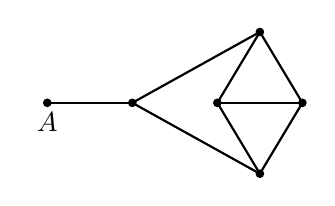
\begin{tikzpicture}[scale = .9]
        \draw[black, thick] (-0.8, 0) -- (-2,0);
        \draw[black, thick] (-0.8, 0) -- (1,1);
        \draw[black, thick] (0.4, 0) -- (1,1);
        \draw[black, thick] (1.6, 0) -- (1,1);
        \draw[black, thick] (-0.8, 0) -- (1,-1);
        \draw[black, thick] (0.4, 0) -- (1,-1);
        \draw[black, thick] (1.6, 0) -- (1,-1);
        \draw[black, thick] (0.4, 0) -- (1.6,0);
        \filldraw[black] (-0.8,0) circle (1.5pt);
        \filldraw[black] (0.4,0) circle (1.5pt);
        \filldraw[black] (1.6,0) circle (1.5pt);
        \filldraw[black] (-2,0) circle (1.5pt) node[anchor = north] {$A$};
        \filldraw[black] (1,-1) circle (1.5pt);
        \filldraw[black] (1,1) circle (1.5pt);
  			 %\node at (-2, 0) {\small{$A$}}; 
    \end{tikzpicture}
		\vspace*{2mm}
    \caption{A gadget that can be attached to a degree one or two vertices
		(at the point $A$) in a max degree $3$ graph to make all vertices have
		degree $3$. With each addition of the gadget, we increase the vertex 
		cover by a size of $3$, regardless of whether $A$ is part of a vertex 
		cover.}
    \label{fig:osg-structure-hook}
\end{figure}

The reduction first makes $G$ $3$-regular by attaching (one or two of) the 
gadget shown in ~\ref{fig:osg-structure-hook} to $v \in G$ that are not 
degree $3$. This results in a $3$-regular graph $G'$. For each attached 
gadget, $k$ is bumped up by $3$, i.e., we let $k'$ for $G'$ be $k' = k 
+ 3(3|V(G)| - 2|E(G)|)$. It is straightforward to see that $G$ has a vertex 
cover size of $k$ if and only if $G'$ has a vertex cover size of $k'$.

\begin{figure}[!ht]
    \centering
    \raisebox{10mm}
    {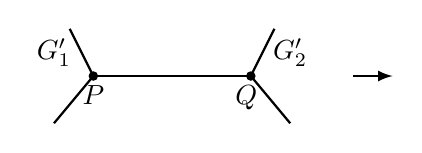
\begin{tikzpicture}
        \draw[black, thick] (-1,0) -- (1,0);
        \draw[black, thick] (-1,0) -- (-1.3,0.6);
        \draw[black, thick] (-1,0) -- (-1.5,-0.6);
        \draw[black, thick] (1,0) -- (1.3,0.6);
        \draw[black, thick] (1,0) -- (1.5,-0.6);
        \draw[black, thick, -latex] (2.3, 0) -> (2.8,0);
        \filldraw[black] (-1.5,0) node[anchor=south] {$G_1'$};
        \filldraw[black] (1.5,0) node[anchor=south] {$G_2'$};
        \filldraw[black] (-1,0) circle (1.5pt) node[anchor=north] {$P$};
        \filldraw[black] (1,0) circle (1.5pt) node[anchor=north] {$Q\,\,$};
    \end{tikzpicture}
    }
    % \hfill
    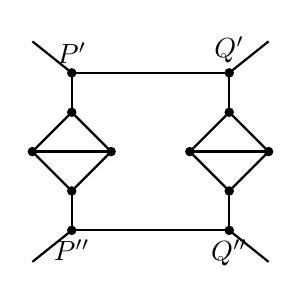
\begin{tikzpicture}
        \coordinate(p1) at (-1.5, 0);
        \coordinate(p2) at (-0.5, 0);
        \coordinate(p3) at (-1, 0.5);
        \coordinate(p4) at (-1, -0.5);
        
        \coordinate(p5) at (-1, 1);
        \coordinate(p6) at (-1, -1);
        
        \coordinate(p7) at (-1.5, 1.4);
        \coordinate(p8) at (-1.5, -1.4);

        \coordinate(q1) at (0.5, 0);
        \coordinate(q2) at (1.5, 0);
        \coordinate(q3) at (1, 0.5);
        \coordinate(q4) at (1, -0.5);

        \coordinate(q5) at (1, 1);
        \coordinate(q6) at (1, -1);
        \coordinate(q7) at (1.5, 1.4);
        \coordinate(q8) at (1.5, -1.4);
        
        \draw[black, thick] (p1) -- (p2);
        \draw[black, thick] (p1) -- (p3);
        \draw[black, thick] (p1) -- (p4);        
        \draw[black, thick] (p2) -- (p3);
        \draw[black, thick] (p2) -- (p4);
        \draw[black, thick] (p6) -- (p4);
        \draw[black, thick] (p5) -- (p3);
        

        \draw[black, thick] (q1) -- (q2);
        \draw[black, thick] (q1) -- (q3);
        \draw[black, thick] (q1) -- (q4);        
        \draw[black, thick] (q2) -- (q3);
        \draw[black, thick] (q2) -- (q4);
        
        \draw[black, thick] (q6) -- (q4);
        \draw[black, thick] (q5) -- (q3);
        
        \draw[black, thick] (q5) -- (p5);
        \draw[black, thick] (q6) -- (p6);
        
        \filldraw[black] (p1) circle (1.5pt);
        \filldraw[black] (p2) circle (1.5pt);
        \filldraw[black] (p3) circle (1.5pt);
        \filldraw[black] (p4) circle (1.5pt);
        \filldraw[black] (p5) circle (1.5pt) node[anchor=south] {$P'$};
        \filldraw[black] (p6) circle (1.5pt) node[anchor=north] {$P''$};
        
        \filldraw[black] (q1) circle (1.5pt);
        \filldraw[black] (q2) circle (1.5pt);
        \filldraw[black] (q3) circle (1.5pt);
        \filldraw[black] (q4) circle (1.5pt);
        \filldraw[black] (q5) circle (1.5pt) node[anchor=south] {$Q'$};
        \filldraw[black] (q6) circle (1.5pt) node[anchor=north] {$Q''$};
        
        \draw[black, thick] (p5) -- (p7);
        \draw[black, thick] (p6) -- (p8);
        \draw[black, thick] (q5) -- (q7);
        \draw[black, thick] (q6) -- (q8);
        
    \end{tikzpicture}
    \vspace{.5mm}
    \caption{Transformation that removes bridge $PQ$ and does not introduce new bridges.
    The minimum vertex cover number is increased by $6$ after each transformation.}
    \label{fig:osg-rmbridge}
\end{figure}

In the second and last step, we remove bridges in $G'$. As in 
~\ref{fig:osg-rmbridge}, for a bridge $PQ$ that divides $G'$ into $G_1'$ 
(containing $P$) and $G_2'$ (containing $Q$), we split the bridge edge 
$PQ$ using the illustrated transformation, which yields a new graph $G''$
that is planar, bridgeless, and $3$-regular, after all bridges are removed
this way. For each such augmentation, the size of the vertex cover is 
bumped up by six. Let $br(G')$ be the number of bridges in $G'$, $G'$ has 
a vertex cover of size  $k'$ if and only if $G''$ has a vertex cover 
of size $k'' = k'+6br(G')$. This completes the proof. 
\end{proof}


\subsection{Hardness on Optimally Guarding a $3$-Net}\label{complexity:osg-3netcomp}
Starting from a planar cubic graph $G$, we construct a structure that we call 
$3$-net, $T_G$, as follows. 
%
First, similar to \cite{feder1988optimal}, to embed $G$ into the plane, 
an edge $uw \in E(G)$ is converted to an odd length path $uv_1, v_1v_2, 
\ldots, v_{2m}w$ where $m > 3$ is an integer. We note that $m$ is different
in general for different edges of $G$. 
%  to be decided later. 
Denote such a path as $u\cdots w$; each edge along $u\cdots w$ is straight 
and has unit edge length. We also require that each path is nearly straight 
locally. 
% This point will be made more precise later.
%
For a vertex of $G$ with degree $3$, e.g., a vertex $u \in V(G)$ 
neighboring $w, x, y \in V(G)$, we choose proper configurations and lengths for 
paths, $u\cdots w$, $u\cdots x$, and $u\cdots y$ such that
these paths meet at $u$ forming pairwise angles of $2\pi/3$. We denote the 
resulting graph as $G'$, which becomes the {\em backbone} of the 
$3$-net $T_G$. 

From here, a second modification is made which completes the 
construction of $T_G$. In each previously constructed 
path $u\cdots w = uv_1\ldots v_{2m}w$, for each $v_iv_{i+1}$, $1 \le i
\le 2m-1$, we add a line segment of length $\sqrt{3}$ that is 
perpendicular to $v_iv_{i+1}$ such that $v_iv_{i+1}$ and the line 
segment divide each other in the middle. A graphical illustration is
given in ~\ref{fig:osg-path-bar}. 
% We note that the bars do not need to be connected to the backbone $G'$. 
$G'$ and the bars form the 
$3$-net, which we denote as $T_G$. An example of transforming $K_4$
into a {\em 3-net} is given in ~\ref{fig:osg-3-net}.

\begin{figure}[ht]
% \vspace*{-4mm}
    \centering
		\vspace*{1mm}
    \includegraphics[scale=0.3]{chapters/osg/figures/edgepath-eps-converted-to.pdf}
		\vspace*{3mm}
% \vspace*{-4mm}
    \caption{Structure within the odd length path and attached 
		perpendicular ``bars'' with length $\sqrt{3}$. Regarding the 
		representation of such non-integral coordinates in the problem 
    input, 
    we may scale the coordinates to some certain extent and
    round them to integers so that the relative distance between
    each other is precise enough
    for the proof.
    % a precise enough fractional representation is enough 
    % for the proof due to the inapproximability gap in the result.
    }
		\vspace*{-1mm}
    \label{fig:osg-path-bar}
\end{figure}

\begin{figure}[ht]
    \centering
    % \vspace*{-8mm}\
    \raisebox{14mm}{
    \begin{overpic}[scale=0.2]{chapters/osg/figures/k4-eps-converted-to.pdf}
      % \put(53,36){\color{black}$w$}
      \put(115,23){$\to$}
      \end{overpic}
    }
      \begin{overpic}[scale=0.4]{chapters/osg/figures/k4_after-eps-converted-to.pdf}
        \end{overpic}
    \caption{Illustration of a $3$-net obtained from $K_4$, the complete graph on 
		$4$ vertices.}
    % \caption{A $3$-net constructed over the backbone in ~\ref{fig:backbone}.
        % \textcolor{red}{Siwei: update this to be based on $G'$ from ~\ref{fig:backbone}}
        % }
    \label{fig:osg-3-net}
\end{figure}

Let $L$ be the number of (unit length) edges of $G'$ (i.e., $L = 
\sum_{uv \in E(G)}len(u\cdots w)$). 
\begin{lemma}\label{l:osg-bl}
A planar bridgeless $3$-regular graph $G$ has a vertex cover of size 
$k$ if and only if its transformed 3-net $T_G$ can be covered
by $K = k + (L-|E(G)|)/2$ circles of radius approximately $\alpha = 1.152$.
\end{lemma}
\begin{proof}
If $G$ has a vertex cover of size $k$, then we put $k$ circles of radius $1$
at the centers of the corresponding vertices in $T_G$. 
%
For each odd length path $u\cdots w$, since either $u$ or $w$ is already 
selected as the circle center, applying one coverage pattern shown
in ~\ref{fig:osg-pathcover} with $(len(u\cdots w) - 1)/2$ circles will cover 
the rest of $u\cdots w$ and all bars on it. So, the total number of circles
used is $K$ to cover all of $T_G$. 

\begin{figure}[!ht]
  \vspace*{0mm}
      \centering
      \includegraphics[scale=0.3]{chapters/osg/figures/edgepath1-eps-converted-to.pdf}\vspace{3mm}
      % \hfill
      \includegraphics[scale=0.3]{chapters/osg/figures/edgepath2-eps-converted-to.pdf}
  \vspace*{0mm}
     \caption{Two coverage patterns on an odd length path with robots of 
      range sensing radius $1$ which is less than $\alpha$.}
      \label{fig:osg-pathcover}
  \end{figure}
  
  \begin{figure}[!ht]
    \centering
    \includegraphics[scale=0.33]{chapters/osg/figures/edgepath3-eps-converted-to.pdf}
  \vspace*{1mm}
    \caption{Asymmetrical coverage of $4$ endpoints requiring a circle of 
    radius at least $2\sqrt{3}/3\approx 1.155$.}
    \label{fig:osg-pathcovert}
  \end{figure}

The ``if'' part requires more analysis. Consider $T_G$ that can be covered 
by $K$ circles of radius $r \approx \alpha$. For a path $u\cdots w$ on $T_G$ whose 
length is $2m+1$, there are $2m-1$ vertical bars associated with it. Consider 
the $4m-2$ endpoints of these vertical bars. We note that (as shown in 
~\ref{fig:osg-pathcovert}), it requires a radius of $2\sqrt{3}/3\approx 1.155$ 
for a circle to cover $4$ bar endpoints in an asymmetrical manner (three endpoints
on one side of the path, one on the other). Since 
we set the radius of coverage circle to be about $\alpha = 1.152$ (actually, 
between $1.152$ and $1.153$),
a circle may only cover up to $4$ bar endpoints. When a circle does cover $4$ 
bar endpoints, it must use a symmetrical coverage pattern, i.e. $4$ endpoints
on two bars, resulting in fully covering two bars. For the 
rest of the proof, we use ``circle'' to mean circles with a radius of $\alpha$,
unless otherwise stated explicitly. 

Since there are $4m - 2$ bar endpoints, it requires $m$ circles to cover all 
bar endpoints when $m \ge 3$. Moreover, at least one circle must cover $4$ 
bar endpoints by the pigeonhole principle. Fixate on such a circle $S$, which 
must have symmetric coverage, we examine the bars on one side of it, say the 
left side, assuming the path $u\cdots w$ is horizontal. If there are more 
than two bars to the left, then it is always beneficial to cover the two bars 
immediately to the left of $S$ using another circle. To see that this is the 
case, look at the two bars ($DE$ and $FH$) and the two associated unit 
length edges ($AB$ and $BC$) to the left of $S$ in ~\ref{fig:osg-two-bar}.
It can be computed that the circle $S$ to the right can cover a maximum 
length of $0.412$ of $AB$ to $A'$. Circles to the left of $S$ then must cover 
$A'B$. Let the circle covering $A'$ be $S'$. We may assume that 
$S'$ covers at least one of $D$ and $E$ (otherwise, at least one more circle 
$S''$ must be added that fall between $S'$ and $S$, in which case $S''$ 
must also cover $A'$). 

  \begin{figure}[ht]
  \vspace*{0mm}
    \centering
     \begin{overpic}[width=0.7\columnwidth]{chapters/osg/figures/two-bar-notext-eps-converted-to.pdf}
     \put(95, 31){$S$}
     \put(62.5,13){$A$}
     \put(50,22.5){$A'$}
     \put(44.3,13){$B$}
     \put(27,13){$C$}
     \put(57.5,36){$D$}
     \put(57.5,0){$E$}
     \put(41,32){$F$}
     \put(41,1.5){$H$}
     \put(14,26){$S'$}
     \end{overpic}
  \vspace*{3mm}
    \caption{When there are enough bars left, it is always better to cover
		two bars at a time with a circle. Two extremal cases of $S'$ covering
		$A'$ and $D$ but not $E$ are shown (as dashed circles), which amounts 
		to rotating the circle $S'$ around $D$.}
    \label{fig:osg-two-bar}
  \end{figure}

If $S'$ covers $A'$ and only one of $D$ or $E$, say $D$, some other circle 
$S''$ must cover $E$. In this case, the coverage region of $S'$ and $S''$ are 
bounded by circles of radius approximately $2.304$ with center at $D$ and $E$, 
respectively. It is readily observed that $S'$ and $S''$ can reach at most one 
more bar to
the left of $FH$ (we note that $S'$ and $S''$ will not be able reach structures
on the $3$-net beyond $u\cdots w$ path). In this case, we can instead move $S'$ 
cover $A'C$, $DE$, and $FH$, and move $S''$ cover the bar to the left of $FH$ 
and potentially one more bar. Therefore, we may assume that $S'$ covers bar 
endpoints $D, E, F$, and $H$, symmetrically along the $u\cdots w$ path. 
Following the reasoning, we may assume that all bars on paths are covered, 
two at a time by a circle in a symmetrical manner, until there are one or two 
bars left before a path reaches a junction where it meets other paths. 

Because there are odd number of bars on a path, the symmetric coverage pattern 
extends until one side of a path has two bars remaining while the other side
has one bar. $m - 2$ circles have been used so far, which means that at least 
two more circles are needed to cover the remaining three bars. Without loss of 
generality, assume two bars out of these three are adjacent and are on the left 
end of $u\cdots w$ and one is on the right. Denote these bars as $b_1, b_2$, 
and $b_3$, from left to right. We call the end of a path with two bars the 
{\em even end} (e.g., the side ending with two bars $b_1$ and $b_2$) and the 
end of the path with one bar the {\em odd end} (e.g., the side ending with one 
bar $b_3$). 

We now examine the coverage of $b_2$ (see ~\ref{fig:osg-end-two-bar} where 
$b_1$ corresponds to $CD$ and $b_2$ corresponds to $AB$). Again, if the two 
endpoints $A$ and $B$ of $b_2$ are covered by more than one circle, then one 
of these two circles can be replaced with one that fully covers $b_1$ and 
$b_2$ (the solid circle in ~\ref{fig:osg-end-two-bar}), since a circle 
covering only one endpoint of $b_2$ (e.g., $B$) will not be able to reach 
structures outside $u\cdots w$. By now, $m-1$ circles have been used and to 
cover $u \cdots w$, at least two more circles are needed at the two ends 
(i.e., $m+ 1$ circles are required to cover $u\cdots w$). 

  \begin{figure}[ht]
    \centering
     \begin{overpic}[width=0.6\columnwidth]{chapters/osg/figures/end-two-bar-notext-eps-converted-to.pdf}
     \put(18, 28.5){$u$}
     \put(64.5, 43){$A$}
     \put(60, 10){$B$}
     \put(51, 39){$C$}
     \put(51, 15.5){$D$}
     \put(68,10){\rotatebox{-12}{{\small $r=2.304$}}}
		 \end{overpic}
  \vspace*{1mm}
    \caption{When there are two bars at the end of a path, it is preferred
		to cover them with a single circle (in red). The dotted circle shows that 
		a circle of radius $2*\alpha$ covering $B$ will not be able to reach 
		structures outside $u\cdots w$.}
    \label{fig:osg-end-two-bar}
  \end{figure}


Next, instead of examining $b_3$, we examine the possible configurations at 
junctions where paths meet. There are four possible cases that contains 
$0$-$3$ odd ends. For the case where only even ends meet, one additional 
circle is needed to cover the rest of the junction 
(~\ref{fig:osg-junction}(a)). When there is one odd end and two even ends 
(~\ref{fig:osg-junction}(b)), it requires one more circle to cover the 
junction. This constraint is how the radius $\alpha = 1.152$ is obtained 
(more precisely, with circles with radius 1.153, no additional circles are 
needed at the junction). When there are two odd ends and one even end 
(~\ref{fig:osg-junction}(c)), at least one more circle is needed to cover 
the the junction. For the last case (~\ref{fig:osg-junction}(d)), no 
additional circles are needed. The cases where additional cycles are needed 
correspond to the junction vertex being selected as a vertex cover. 
It is straightforward to observe that the constructed vertex cover is a valid 
one. The cover has size of $K-(L-|E(G)|)/2$. 

\begin{figure}[!ht]
	\vspace*{4mm}
  \centering
  \hspace{-10mm}
\begin{overpic}[scale=0.66]{chapters/osg/figures/junction-eps-converted-to.pdf}
  \put(16, 0){(a)}
  \put(40, 0){(b)}
  \put(64, 0){(c)}
  \put(88, 0){(d)}
\end{overpic}
\vspace*{2mm}
  \caption{The four possible patterns at the junction using circles of radius 
	less than $\alpha = 1.152$. When we increase the radius to $r = 1.152259$, 
	circles shown in (b) and (c) can successfully cover the junction and the odd 
	ends.}
  \label{fig:osg-junction}
\end{figure}
\end{proof}

It is clear that Lemma~\ref{l:osg-bl} holds for discs with radius in 
$[1, \alpha)$. Thus, approximating $size(T_G, K)$ to less than a 
factor of $\alpha$ will decide whether $G$ has a vertex cover of 
$k$, yielding the hard-to-approximate result.
Also, it can be observed that all lengths are polynomial with respect to 
the problem input size, which implies strongly NP-hardness.
\begin{theorem}\label{t:osg-3nethard}
The minimum radius for cover a $3$-net using 
% $(({L-|E|})/{2}+k)$ 
$k$ circular discs 
% while minimizing the maximum disc radius 
is strongly NP-hard to approximate within a 
factor of $\alpha = 1.152$.
\end{theorem}


\subsection{From $3$-Nets to Simple Polygons}\label{subsec:osg-osgthard}
We proceed to show that \osgt is hard to approximate for a simply polygon 
by converting a $3$-net into one. Along the backbone $G'$ of a $3$-net 
$T_G$, we first expand the line segments by $\delta$ to get a 2D region  
(see ~\ref{fig:osg-door}(a)). We may describe the interior of the resulting 
polygon as 
\vspace*{-1mm}
\[P=\{p\in \R^2\ |\ \min_{q\in T_G}(\lVert p-q\rVert_1)\leq \delta/2\}\]
\vspace*{-4mm}

For small enough $\delta$, it's clear that $P$ is a polygon with holes.
Let $K = (({L-|E|}){2}+k)$, it holds that
\vspace*{-1mm}
\begin{align*}
&size(K, T_G) \leq               size(K, P)\leq size(K, T_G) + \delta,\\
&size(K, T_G) \leq      size(K, \partial P)\leq size(K, T_G) + \delta.
\end{align*}
\vspace*{-5mm}

To convert the structure into a simple polygon, we can open ``doors'' of 
width $\delta$ on the structure to get rid of the holes (see 
~\ref{fig:osg-door}(b)). Each opening removes one hole from $P$. This is 
straightforward to check; we omit the details. 
\begin{figure}[ht]
		\centering
		\vspace*{0mm}
    \begin{small}
    \includegraphics[scale=.3]{chapters/osg/figures/holes-eps-converted-to.pdf} 
    \hspace{1in}
    \begin{overpic}[scale=.3]{chapters/osg/figures/doors-eps-converted-to.pdf}
        \put(50,42){$\delta$}
        \put(-75,3){(a)}
        \put(46,3){(b)}
    \end{overpic}
	  \end{small}
		\vspace*{1mm}
    \caption{(a) A $3$-net $T_G$ maybe readily converted into a simple polygon 
		$P$ with holes by expanding along its backbone. (b) Creating a ``door'' 
		of width $\delta$ will remove one hole from $P$.}
    \label{fig:osg-door}
\end{figure}

Denoting the resulting simple polygon as $P'$, we have
\vspace*{-1mm}
\begin{align*}
&size(K, P) - \delta  \leq               size(K, P')\leq size(K, P),\\
&size(K, \partial P) - \delta  \leq      size(K, \partial P')\leq size(K, \partial P).
\end{align*}
\vspace*{-5mm}

Therefore, both $size(k, P')$ and $size(k, \partial P')$ are between 
$size(k, T_G) - \delta$ and $size(k, T_G) + \delta$. Suppose the \osgt for 
$\partial P'$ or $P'$ has a polynomial approximation algorithm with 
approximation ratio $1.152 - \varepsilon$ where $\varepsilon > 0$, let $\delta = 
\varepsilon/2$, then the optimal guarding problem for the $T_G$ can 
be approximated within 1.152 disobeying the inapproximability gap by 
Theorem~\ref{t:osg-3nethard}. Therefore,

\begin{theorem}\label{t:osg-osgthard}
\osgt is NP-hard and does not admit a polynomial time approximation 
within a factor of $\alpha$ with $\alpha = 1.152$, unless 
P$=$NP.
\end{theorem}

\subsection{\opgt with Sensor Guarding Restrictions}\label{subsec:osg-2-seghard}
The inapproximability gap from Theorem~\ref{t:osg-osgthard} prompts us to 
further consider restrictions on the setup with the hope that meaningful 
yet more tractable problems may arise. On natural restriction is to 
limit the number of continuous segments a mobile sensor may cover. As 
will be shown in Section~\ref{subsec:osg-singleseg}, if a mobile sensor may 
only guard a single continuous perimeter segment, a 
$(1 + \varepsilon)$-optimal solution can be computed efficiently. 
On the other hand, it turns out that if a sensor can guard up to two 
continuous perimeter segments, \opgt remains hard to approximate. 

\begin{theorem}\label{them:osg-twoconthard}
\opgt of a simple polygon cannot be approximated within $\alpha\approx 1.152$ 
even when each robot can guard no more than two continuous boundary segments,
unless P$=$NP.
\end{theorem}
\begin{proof}
Due to \cite{petersen1891}, every bridgeless $3$-regular graph $G$ has a 
perfect matching. We can obtain such a perfect matching of the $3$-regular 
graph using Edmonds' Blossom algorithm in polynomial time\cite{edmonds_1965}. 
Doubling the edges in the perfect matching, we can then obtain a 4-regular 
graph $G'$. 

\begin{figure}[ht]
		\vspace*{-2mm}
    \centering
    \includegraphics[scale=0.3]{chapters/osg/figures/1going-eps-converted-to.pdf}\hspace{2mm}
	  \begin{overpic}[scale=.3]{chapters/osg/figures/2going-eps-converted-to.pdf}
        \put(-55,-10){(a)}
        \put(49,-10){(b)}
    \end{overpic}
		\vspace*{6mm}
    \caption{(a) Part of the augmented Eulerian path for non-doubled 
		paths. (b) Part of the augmented Eulerian path for doubled paths.}
    \label{fig:osg-path_exp}
		\vspace*{-1mm}
\end{figure}

The Eulerian tour on $T_G$ may have self-intersections, which 
will prevent the tour from being a simple polygon. To address this, we may use 
one of two possible solutions outlined in ~\ref{fig:osg-eliminter} to eliminate
the self-intersections. 
\begin{figure}[ht]
    		\vspace*{2mm}
				\centering
	  \begin{overpic}[width=\columnwidth]{chapters/osg/figures/t345-eps-converted-to.pdf}
        \put(12,-6){(a)}
        \put(48,-6){(b)}
        \put(84,-6){(c)}
    \end{overpic}
		\vspace*{3mm}
        \caption{In order to eliminate possible self-intersections in 
				(a), we may transform it into one of the solutions given in 
				(b) and (c) to make the Eulerian tour remain connected (one 
				of the two solutions will satisfy this).}
        \label{fig:osg-eliminter}
\end{figure}

At this point, we readily observe that Theorem~\ref{t:osg-osgthard} applies. 
Furthermore, an optimal solution always allows each mobile sensor to 
cover only two continuous perimeter segments. This is clear in the middle 
of any paths of $T_G$; at junctions, the polygon boundary will be either 
one of two possibilities shown in ~\ref{fig:osg-2types}, where a sensor
again covers at most two continuous segments of the simple polygon. 
\begin{figure}[!ht]
    \centering
    \includegraphics[scale=.29]{chapters/osg/figures/t1-eps-converted-to.pdf}
    \includegraphics[scale=.29]{chapters/osg/figures/t2-eps-converted-to.pdf}
    \caption{The figure shows two possible types of boundaries near a 
		vertex with degree of $4$. A robot near the vertex will only be able 
		to cover two disjoint but individually continuous boundary segments 
		with sensing radius less than $\alpha$ if the solution is to be optimal.}
    \label{fig:osg-2types}
\end{figure}
\end{proof}


\section{Effective Algorithmic Solutions for \osgt}\label{sec:algo}
\def\algomed{\textsc{Min\_Enclose\_Disc}\xspace}
In this section, we present several algorithmic solutions for \osgt. 
First, a fully polynomial approximation scheme (FPTAS)
is presented that solve \opgt with the additional requirement 
that each sensor is responsible for a continuous perimeter segment. 
This contrasts Theorem~\ref{them:twoconthard}. Then, we show that 
there exist polynomial time algorithms that readily guarantee a
$(2+\varepsilon)$-approximation for \osgt. This is followed by an 
integer linear programming (ILP) method that delivers high-quality
solutions (as compared with the $(2 + \varepsilon)$-approximate one)
and has good scalability. 

In preparation for introducing the result, we first describe a method
that is used for discretizing the problem. For a simple polygon $P$, 
we can approximately represent its boundary $\partial P$ as a set of 
balls with radius $\varepsilon$ along $\partial P$, by splitting  
$\partial P$ into $N=\lceil{len(\partial P)}/({2\varepsilon})\rceil$ 
continuous pieces of length at most $2\varepsilon$ and putting the balls' 
centers at their midpoints. 
%
Denote set of $\varepsilon$-balls as $S_B$, and the set of their centers 
as $S_O=\{o_1,\dots, o_N\}$. Since it holds that $size(k,\partial P) \leq 
size(k, S_B) \leq size(k, S_O) + \varepsilon \leq size(k, \partial P) 
+ \varepsilon$, the minimum coverage radius of the discritized version 
of covering $S_O$ will differ no more than $\varepsilon$ from the original 
problem of covering $\partial P$. Similarly, for covering the interior 
of $P$, we can put $P$ into a grid with cell side length $\varepsilon$, 
and set the center of the grid cells intersecting with $P$ as $S_O$, 
creating at most $N=O(({len(\partial P)}/{\varepsilon})^2)$ samples. 
The discretization process converts guarding $P$ or $\partial P$ to 
guarding $S_O$. 

\subsection{\opgt with Single Segment Guarding Limitation}\label{subsec:singleseg}
By Theorem.~\ref{them:twoconthard}, if a mobile sensor can guard up to two 
continuous perimeter segments, \osgt is hard to approximate within 
$1.152$-optimal. 
Translating this into guarding elements of $S_O$, this means that a sensor
can guard two {\em chains} of elements from $S_O$, where each chain contains 
some $m$ elements $o_1, \ldots, o_m$ that are neighbors along $\partial P$. 
Interestingly, if each sensor may only guard a single chain of elements 
from $S_O$, we may compute an optimal cover for $S_O$ using $O(N^2 \log N)$ 
time. This readily turns into a fully polynomial time approximation scheme 
(FPTAS) for \opgt. 
% based on efficent implementation of the expected linear time 
% implementation to get the Minimum Enclosing Disc of a set of points \cite{welzl1991smallest}\cite{Mark1997computation}.  
The algorithm operates by checking multiple times whether a given radius 
$r$ is sufficient for $k$ discs of the given radius to cover elements of 
$S_O$ where each disc covers only a single chain of elements. 

A single feasibility check is outlined in Algorithm~\ref{algo:cont}.
In the pseudo code, it is assumed that the indices are modulo $N$, e.g. 
$M[N+1] = M[1]$, $o_{N+1} = o_1$. 
%
Algorithm~\ref{algo:cont} is based on an efficient implementation of 
a subroutine \algomed (from e.g., \cite{welzl1991smallest,
Mark1997computation}) that computes the disc with minimum radius to 
enclose a given set of points in expected linear time. With this, a sliding 
window can be applied to find the rightmost $end$ for each $1\leq i\leq 
N$ such that $o_i, \dots, o_{end}$ can be enclosed in a circle of radius 
$r$. The length of this sequence is stored in $M[i]$. 

As $o_{end}$ cannot come around and meet $o_i$, the total call to 
\algomed is no more than $2N$. After this, the algorithm simply tries to put 
discs from each $o_i$ to cover as many centers as possible to see 
whether $S_O$ can be enclosed with $k$ discs. An optimization can be made 
by only examining starting point as $o_1, \dots, o_{M[1]+1}$, since there 
is no circle of radius of $r$ that can cover them together by the 
definition of $M$.
%
The apparent complexity of Algorithm~\ref{algo:cont} is $O(N^2)$. Since 
there are a total of $N$ points and $k$ robots, in a majority 
of cases a circle would enclose about $N/k$ points, which effectively 
lowers the time complexity to $O(N^2/k)$.

\def\algoptfeasi{\textsc{Opg\_2D\_Cont\_Feasible}}
\SetKw{Continue}{continue}
\SetKw{True}{true}
\SetKw{False}{false}
\begin{algorithm}
\begin{small}
\DontPrintSemicolon
\SetKwComment{Comment}{\%}{}
\caption{\textsc{Opg\_2D\_Cont\_Feasible}}    %($P$, $k$, $r$, $\varepsilon$)}}
\label{algo:cont}
\SetKwInOut{Input}{Input}
\SetKwInOut{Output}{Output}
\KwData{$S_O=\{o_1, \dots, o_N\}$, sample points in circular order\\
\qquad\quad$k$, the number of robots\\
\qquad\quad $r$, the candidate sensing radius}
\KwResult{\True or \False, indicating whether $S_O$ can be covered with k discs with radius $r$}
\vspace{2mm}

\If{{\sc Min\_Enclose\_Disc}($o_1, \dots, o_N$)$\leq r$} {\Return{\True}}
\vspace{1.5mm}

\Comment{\small Phase 1: find the maximum number of consecutive points a disc of radius $r$ can enclose
from each $c_i$.}%$arr[i]$ \small stores the number of continuous points the disc can enclose from $c_i$.}
\vspace{1.5mm}

$M\leftarrow$ an array of length $N$; $end\leftarrow 1$;\;
\vspace{1.5mm}

\For{$i=1$ \KwTo N}{
\While{{\sc Min\_Enclose\_Disc($o_i, \dots, o_{end+1}$) $\leq r$ }}{
    $end\leftarrow end+1$;\;
}
$M[i]\leftarrow end - i + 1$;\;
}
\vspace{1.5mm}

\Comment{\small Phase 2: try to tile from each $o_i$.}
\vspace{1.5mm}

\For{$i=1$ \KwTo $N$}{
$j \leftarrow i$, \quad $cnt \leftarrow k$;\;
\While{$cnt > 0$}{
    $j \leftarrow j + M[j]$;\;
    \If{$j-i \geq N$}{\Return{\True}}
    $cnt\leftarrow cnt-1$\;
}
}
\Return{\False}
\end{small}
\end{algorithm}



Note that for the optimal coverage radius $r^*$, it holds that $r_{min} = 
0 < r^* \leq {len(\partial P)}/({2k}) = r_{max}$. 
Recall that $N=\lceil len(\partial P)/(2\varepsilon)\rceil$.
Hence, after at most 
\[
  \log\frac{r_{max} - r_{min}}{\varepsilon} = \log(\frac{len(\partial P)}{2k\varepsilon})  = O(\log\frac{N}{k} )
\]
times of binary search on the optimal radius $r^*$ by calling \algoptfeasi, 
the search range of $r^*$ or the gap between $r_{max}$ and $r_{min}$ will 
be reduced to within $\varepsilon$. So, it takes expected $O(N^2 \log (N/k))$ 
time in total to get an approximate solution with radius at most $\varepsilon$ 
more than $size(k, S_O)$ or $size(k, \partial P)$.
\begin{theorem}\label{t:opgtsseg}
    Under the rule of continuous coverage, \opgt for a simple 
		polygon can be approximated to $(1 + \varepsilon)$-optimal in expected 
		$O(N^2\log N)$ time, and $O(({N^2}/{k} )\log(N/k))$ in most cases,
    where $N=\lceil{len(\partial P)}/({2\varepsilon})\rceil$.
\end{theorem}

\remark{In the running time complexity analysis, we implicitly 
used the assumption that $len(\partial P)$ is polynomial to problem input 
size (see Section~\ref{sec:problem}). Also, the algorithm given above
computes an $OPT + \varepsilon$ optimal solution. However, 
% due to the 
it can be naturally assumed that the optimal
sensing radius $OPT$ is lower bounded in realistic scenarios. 
So, an $(OPT + \varepsilon)$ solution
directly translates into a $(1 + \varepsilon)$-optimal solution. 
Lastly, using techniques similar to those from \cite{FenHanGaoYuRSS19,FenYu2020RAL}, 
we mention that results in this subsection readily extends to multiple 
simple polygons with gaps along the boundary. 
These arguments continue to apply throughout the rest of  
this section. 
%

Regarding the choice in implementation, the minimum enclosing disc problem 
(1-center problem) also has deterministic solution 
\cite{megiddo1983linear} in linear time, but a randomized algorithm is considered to be 
more efficient\cite{welzl1991smallest} and easier to implement.}

\subsection{$(2 + \varepsilon)$ Approximation}
In dealing with Euclidean $k$-clustering problems, two seminal methods 
are often brought out, both of which compute $2$-approximation solutions
for $k$-center problem in polynomial time. This is fairly close to the 
inapproximability gap of $1.822$ for Euclidean $k$-center
problem\cite{feder1988optimal}. The first 
\cite{hochbaum1985best, vazirani2013approximation} transforms the 
clustering problem to a dominating set problem and then applies parametric 
search on the cluster size (radius), resulting in a $2$-approximation in 
time $O(n^2\log n)$ with $n$ being the number of points to cover. 
A second method \cite{gonzalez1985clustering} takes 
a simpler farthest clustering approach by iteratively choosing the 
furthest point from the current centers as the new center. The method runs 
in $O(nk)$ but is subsequently improved to $O(n\log k)$ in 
\cite{feder1988optimal}. So, by applying either of them on $S_O$, we have

\begin{proposition}
    \osgt can be approximated to $(2 +\varepsilon)$-optimal in polynomial time 
		with $N=O({len(\partial P)}/{\varepsilon})$ samples for perimeter 
		guarding and $N=O(({len(\partial P)}/{\varepsilon})^2)$ samples for
    region guarding.
\end{proposition}

For evaluation, we implemented the farthest clustering approach 
\cite{gonzalez1985clustering}.

\subsection{Grid and Integer Programming-based Algorithm}
Approximation using grids \cite{har2011geometric} often exhibits good 
optimality guarantees and bounded time complexity. Seeing that and knowing
that \osgt is hard in general, we attempted grid-based integer linear programming 
(ILP) methods for solving \osgt with good success. Our ILP model 
construction is done as follows. 

%Grid-based representation
%and approximation, suprisingly, achieve close to optimal solution quality guarentee 
%as well as computational efficiency with nowadays mathematical programming libraries as 
%Gurobi\cite{optimization2019gurobi} or CPLEX \cite{cplex2009v12} etc.

Consider bounding the polygon $P$ of interest by an $m\times n$ square grid 
where each cell is $\varepsilon \times \varepsilon$, and denote $g_{ij}$ as the center 
of the cell at row $i$ and column $j$. If we limit the possible locations of 
each robot to the center of some grid cell, the optimal radius with this 
limitation will only be at most $\sqrt{2}\,\varepsilon / 2$ away from 
$size(k, S_O)$. This could be seen by moving the robot locations in the optimal deployment
to their nearest grid centers respectively and applying triangle inequality.

So, given a candidate radius $r$, to check the feasibility of whether 
$\partial P$ can be covered by $k$ circles of radius $r$, we adapt an 
approach for solving the $k$-center problem\cite{daskin2000new} with 
integer linear programming. Specifically, we create $m\times n$ boolean 
variables $y_{ij}$, $1\leq i\leq m$, $1\leq j \leq n$, indicating whether 
there is a robot at $g_{ij}$, then start to check the feasibility of 
following integer programming model.
\begin{align}
    \sum_{ 1\leq i\leq m }\,\sum_{1\leq j \leq n} y_{ij} \leq k\qquad \qquad \qquad \\
    \sum_{i,\ j\ s.t.\ \lVert g_{ij} - o_\ell\rVert_2\ \leq\ r} y_{ij} \geq 1 \text{ for each }\, 1\leq \ell \leq N\\
    y_{ij} \in \{0,1\}\ \qquad 1\leq i\leq m,\ 1\leq j \leq n
\end{align}
The first constraint says the number of locations is no more than $k$, and 
the second ensures each $o_\ell$ can be covered by at least one circle 
with radius $r$ illustrated in Fig.~\ref{fig:ilpexample}.

\begin{figure}[!ht]
    \centering
		\vspace*{1mm}
		\begin{overpic}[width=1\columnwidth]{chapters/osg/figures/ilp_example-eps-converted-to.pdf}
        \linethickness{0.4mm}
        \put(40.2,25.3){\color{red}\vector(0.8,1.05){15.6}}
        \put(40.2,17){\color{red}\vector(1.45,-1.1){15.5}}
        \put(40,19){\color{blue}$o_{67}$}
        \put(69,24){\color{blue}$o_{67}$}
    \end{overpic}
		\vspace*{1mm}
    \caption{This perimeter guarding example illustrates constraint 
		($2$) for $o_{67}$ with $r=7$. The black dots are the sampled $S_O = 
		\{o_1, \dots, o_{100}\}$. In order to cover $o_{67}$, at least one 
		among the red color grid cell centers need to be selected as robot location.}
    \label{fig:ilpexample}
\end{figure}


When the ILP model has a feasible solution, $r^* = size(k, S_O) \leq r$ 
and $r\leq r^* = size(k, S_O) $ otherwise. This means that we can do a binary 
search on $r^*$, from an initial range of $r^* = size(k, S_O)$: $r_{min}^i=0 
<  r^* \leq {len(\partial P)}/({2k})=r_{max}^i$, until finally $r^f_{max} - 
r^f_{min}$ is reduced to the selected granularity of $\varepsilon$.

\begin{remark}
    With minor modifications, the ILP model applies to 2D region 
		guarding, where the number of constraint $(2)$ will then be $O(mn)$ 
		with one for each grid that intersects with the polygon in an $m\times n$ 
		grid. The initial upper bound set as $r^*$ be $len(\partial P)$ and 
		lower bound set as $\sqrt{{area(P)}/({k\pi})}$. It is also possible to 
		apply the $(2+\varepsilon)$-approximation algorithm and set the result 
		as the initial upper bound with the half of it as the initial lower 
		bound.
\end{remark}


\section{Evaluation and Application Scenarios}\label{sec:expr}
Our evaluation first verifies the algorithms' running time matches 
the claimed bounds. Then, two practical scenarios are illustrated 
to show how \opg may be adapted to applications. 

\vspace*{-1mm}
\subsection{Algorithm Performance}
\vspace*{-1mm}
In the performance results presented here, a data point is the 
average from $10$ randomly generated \opg instances. All algorithms 
are implemented in Python 2.7, and all experiments are executed on 
an Intel\textsuperscript{\textregistered} Xeon\textsuperscript{\textregistered} 
%E5-1660 v3 
CPU at 3.0GHz. % with 32GB RAM.% at 2133MHz.
Some additional performance results can be found in the Appendix.

%\subsubsection{\algoMRSimple} 
For the case of $m$ perimeters each containing a single segment, for 
each $1 \le i \le m$, we set $len(\partial R_i) = 1$ and let $len(P_i)$ 
be uniformly distributed in $(0, 1]$. ~\ref{fig:opg-mpsc-example} shows 
the result for an example with $m = 10$ and $n = 30$. For various values 
of $m, n$, the running time of \algoMRSimple is summarized in 
Table~\ref{eval:opg-mpsc}, which scales very well with $m$ and $n$ (note that 
the $n \le m$ case does not make much sense here). 

\begin{figure}[ht!]
    \vspace*{-3mm}
    \centering
    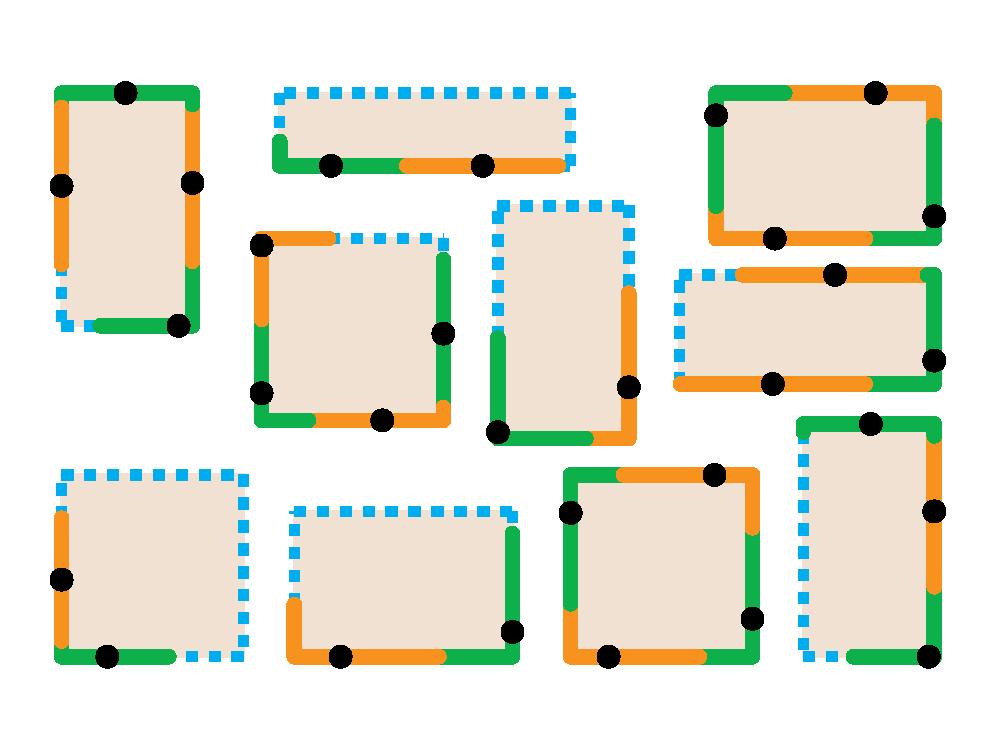
\includegraphics[keepaspectratio, scale=0.32]{./chapters/opg/figures/mpsc-example.eps}
    \vspace*{-6mm}
    \caption{\label{fig:opg-mpsc-example} 
    An example problem instance when $m = 10$ and $n = 30$. The black dots
		indicate deployed robot locations; the green and orange lines indicate
		the coverage.
    %We use blue dashed lines to show the gaps which do not need to be covered. 
    %The black filled circles illustrate final robot deployment locations, and 
    %the orange/green lines demonstrate individual robot covers. 
    %In this example, we use a different distribution to sample $len(P_i)$ due to 
    %cosmetic reasons.
		}
    \vspace*{-2mm}
\end{figure}

\begin{table}[ht!]
    \centering
		\vspace*{-4mm}
    \begin{footnotesize}
    \begin{tabular}{|c|c|c|c|c|c|c|} 
        \hline
        \diagbox{$m$}{$n$}       & $10^8  $ & $10^9   $ & $10^{10}$ & $10^{11}$ & $10^{12}  $ \\ \hline
        %\rule{0pt}{2.5ex} $10^3$ & $0.001 $ & $0.001  $ & $0.001  $ & $0.001  $ & $0.001    $ \\ \hline
        %\rule{0pt}{2.5ex} $10^4$ & $0.006 $ & $0.007  $ & $0.008  $ & $0.008  $ & $0.008    $ \\ \hline
        %\rule{0pt}{2.5ex} $10^5$ & $0.075 $ & $0.088  $ & $0.102  $ & $0.107  $ & $0.106    $ \\ \hline
        \rule{0pt}{2.5ex} $10^6$ & $1.152 $ & $1.442  $ & $1.508  $ & $1.652  $ & $1.617    $ \\ \hline
        \rule{0pt}{2.5ex} $10^7$ & $13.963$ & $17.281 $ & $18.796 $ & $20.354 $ & $20.627   $ \\ \hline
        \rule{0pt}{2.5ex} $10^8$ & NA       & $176.115$ & $223.186$ & $227.250$ & $230.000  $ \\ \hline
    \end{tabular}
		\end{footnotesize}
		% \vspace*{-3mm}
    \caption{\label{eval:opg-mpsc} \algoMRSimple~running time (seconds)}
		% \vspace*{-4mm}
\end{table}

%Recall that when the problem has multiple perimeters with single components, 
%each perimeter has exactly one segment and at most one gap. Our problem 
%generation procedure works as follows: given the number of perimeters $m$, we 
%first generate $m$ rectangles $\{R_1, \dots, R_m\}$ with $len(\partial R_i) = 1$ 
%for all $1 \leq i \leq m$, and then select a closed connected component $P_i$ 
%for each $R_i$. Here, $len(P_i)$ is uniformly randomly sampled from $(0, 1]$. 
%An example problem instance along with its optimal cover is shown in 
%~\ref{fig:mpsc-example}. The computation time of \algoMRSimple~under 
%different $m$ and $n$ is presented in Table.~\ref{eval:mpsc}. 
%\sh{Plots here. The constant factor in the $O(m(\log n + \log m) + \sum_{i} M_i)$ time 
%complexity is around $5 \times 10^{-8}$ seconds. }

For the case of a single perimeter with multiple components, a random 
polygon is generated on which $2q$ points are randomly sampled that 
yield $q$ segments (that form the perimeter) and $q$ gaps. An example 
instance and the optimal solution with $q=3$ and $n = 10$ is illustrated 
in ~\ref{fig:opg-spmc-example}. The computation time for various $q$ and 
$n$ combinations is given in Table~\ref{eval:opg-spmc}.
\begin{figure}[ht!]
    \vspace*{-3mm}
    \centering
    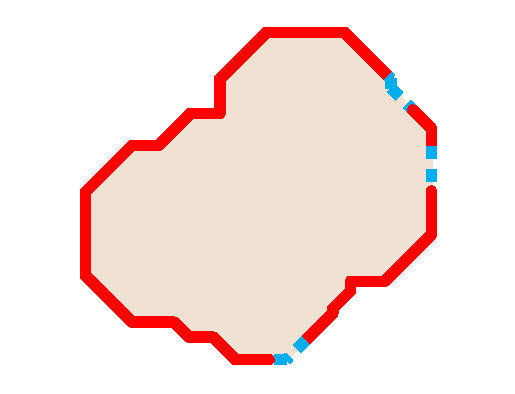
\includegraphics[keepaspectratio, scale=0.4]{./chapters/opg/figures/spmc-example.eps}
    \includegraphics[keepaspectratio, scale=0.4]{./chapters/opg/figures/spmc-solution.eps}
    \vspace*{-3mm}
    \caption{\label{fig:opg-spmc-example} 
    An example problem instance when $q = 3$ and $n = 10$. In this case, the 
		optimal cover actually covers one gap.}
    \vspace*{-4mm}
\end{figure}

\begin{table}[ht!]
    \vspace*{-3mm}
    \footnotesize
    \centering
    \begin{tabular}{|c|c|c|c|c|c|c|} 
        \hline
        \diagbox{$q$}{$n$}       & $10^1   $ & $10^2   $ & $10^3  $  & $10^4   $ & $10^5$   \\ \hline       
        \rule{0pt}{2.5ex} $10^2$ & $0.013  $ & $0.015  $ & $0.016 $  & $0.016  $ & $0.017$  \\ \hline   
        \rule{0pt}{2.5ex} $10^3$ & $1.363  $ & $1.595  $ & $1.622 $  & $1.634  $ & $1.641$  \\ \hline   
        \rule{0pt}{2.5ex} $10^4$ & $159.404$ & $188.497$ & $210.492$ & $212.473$ & $212.780$\\ \hline   
    \end{tabular}
    \vspace*{-3mm}
    \caption{\label{eval:opg-spmc} \algoSRG~computation time (seconds)}
    \vspace*{-4mm}
\end{table}


%\subsubsection{\algoSRG} 
%To generate a problem of a single perimeter divided by interlaced segments and gaps, 
%we first create an arbitrary polygon $R$. Then, we uniformly randomly sample $2q$ points 
%on $\partial R$ to divide it into $q$ segments and $q$ gaps. 
%An example problem instance along with its optimal cover is shown in 
%~\ref{fig:spmc-example}. The computation time of 
%\algoSRG~under different $q$ and $n$ is presented in Table~\ref{eval:spmc}.

For multiple perimeters containing multiple components, $m$ polygons 
are created with $len(\partial R_i)$ randomly distributed in $[1, 10]$. 
For setting $q_i$, we fix a $q$ and let $q_i = q(0.5 + random(0, 1))$. 
Representative computation results of \algoMRG are listed in 
Table~\ref{eval:opg-mpmc}.
%whose perimeters' lengths are uniformly randomly sampled from interval $(1, 10)$. 
%The computation time under different $m$, $q$, and $n$ values are provided in Table~\ref{eval:mpmc}. 
%We observe that with the same $q$, $n$ parameters, the computation time is directly proportional to $m$.
\begin{table}[ht!]
    \vspace*{-2mm}
    \footnotesize
    \centering
    \begin{tabular}{|c|c|c|c|c|c|c|} 
        \hline
        \multirow{2}{*}{$q$} & \multirow{2}{*}{$n$} & \multicolumn{5}{|c|}{$m$} \\ \cline{3-7}
        \rule{0pt}{2.5ex} & & $10$ & $20$ & $30$ & $40$ & $50$ \\ \hline
        %\rule{0pt}{2.5ex} $10^1$ & $10^2$ & $ 0.015$ & $ 0.027$ & $ 0.039$ & $ 0.045$ & $ 0.054$ \\ \hline
        \rule{0pt}{2.5ex} $10^1$ & $10^3$ & $ 0.047$ & $ 0.063$ & $ 0.076$ & $ 0.091$ & $ 0.108$ \\ \hline
        %\rule{0pt}{2.5ex} $10^2$ & $10^2$ & $ 1.492$ & $ 2.784$ & $ 4.168$ & $ 5.404$ & $ 6.444$ \\ \hline
        \rule{0pt}{2.5ex} $10^2$ & $10^3$ & $ 2.191$ & $ 3.771$ & $ 5.523$ & $ 7.707$ & $ 9.369$ \\ \hline
        \rule{0pt}{2.5ex} $10^2$ & $10^4$ & $ 7.105$ & $ 9.619$ & $11.369$ & $12.760$ & $15.107$ \\ \hline
    \end{tabular}
    \vspace*{-3mm}
    \caption{\label{eval:opg-mpmc} \algoMRG~computation time (seconds)}
    \vspace*{-4mm}
\end{table}

Due to limited space, only selected essential performance data is 
presented here. More complete performance data and associate analysis 
can be found in the Appendix. 


\subsection{Two Applications Scenarios}
\noindent\textbf{Securing a perimeter}. As a first application, consider
a situation where a crime has just been committed at the Edinburgh 
Castle (see ~\ref{fig:opg-edinburgh}). The culprit remains in the confines 
of the castle but is mixed within many guests at the scene. As the 
situation is being investigated and suppose that the brick colored 
buildings are secured, guards (either personnel or a number of drones) may 
be deployed to ensure the culprit does not escape by climbing down the 
castle walls. Using \algoSRG, a deployment plan can be quickly computed 
given the amount of resources at hand so that each guard only needs to 
secure a minimum length along the castle walls. ~\ref{fig:opg-edinburgh} 
shows the optimal deployment plan for $15$ guards. 

\begin{figure}[ht]
	\vspace*{-2mm}
	\begin{center}
		\begin{overpic}[width=0.7\textwidth, tics=5]{./chapters/opg/figures/castle_15.eps}
			% \put(82,44){{\small $\W$}}
		\end{overpic}
	\end{center}
	\vspace*{-4.5mm}
	\caption{\label{fig:opg-edinburgh} Optimal deployment of $15$ guards around 
	walls of the Edinburgh Castle. The brick colored structures are buildings 
	that create gaps along the boundary.}
	%\vspace*{-3mm}
\end{figure}

\noindent\textbf{Fire monitoring}. In a second application, consider 
~\ref{fig:opg-forest} where a forest fire has just been put out in 
multiple regions. As there is still some chance that the fire may 
rekindle and spread, for prevention, a team of firefighters is to be 
deployed to watch for the possible spreading of the fire. Here, in 
addition to using \algoMRG to compute optimal locations for deploying 
the firefighters, we also generate minimum time trajectories for the 
firefighters to reach their target locations while avoiding going 
through the dangerous forests. This is done via solving a bottleneck 
assignment problem \cite{burkard1999linear}.
Note that the lake region creates gaps that cannot be traveled by the 
firefighters; this can be handled by making these gaps infinitely large. 
~\ref{fig:opg-forest} shows the optimal locations for $34$ firefighters. 
Animations of the deployment process and other test cases can be found 
in the accompanying video. 

\begin{figure}[ht]
	\vspace*{-2mm}
	\begin{center}
		\begin{overpic}[width=0.7\textwidth,tics=5]{./chapters/opg/figures/forest_solution.eps}
			%\put(82,44){{\small $\W$}}
		\end{overpic}
	\end{center}
	\vspace*{-4.5mm}
	\caption{\label{fig:opg-forest}  Optimal deployment of $34$ firefighters for 
	forest fire rekindling prevention.}
	\vspace*{-3mm}
\end{figure}




\section{Conclusion and Discussions}\label{sec:conc}
In this study, we examine \osgt, the problem of directly computing a deployment 
strategy for covering 1D or 2D critical sets using many mobile sensors while 
minimizing the maximum sensing radius. After showing that \osgt is computationally 
intractable to even approximate within $1.152$, we describe several 
algorithmic solutions with optimality and/or computation time guarantees. 
Subsequent thorough evaluation demonstrates the effectiveness of these algorithmic 
solutions. Finally, we demonstrate the utility of our algorithmic solutions with 
two application scenarios. 
%
Due to space limit, guarding perimeters with gaps (see, e.g.,~\cite{FenHanGaoYuRSS19}) 
is not discussed in this work. However, because our algorithms work with a 
grid-based discretization, the results directly apply to arbitrary bounded 1D and 2D 
sets. 

Many intriguing questions follow; we mention two here concerning the sensing 
capabilities. First, \osgt works with circular regions which is perhaps the simplest one
due to symmetry. What if the sensor region is not circular? Whereas such cases 
appear to be hard \cite{culberson1988covering}, effective scalable solutions may 
still be possible. Secondly, currently we assume that all parts of the critical 
set to be guarded have equal importance. What if certain subsets are more important? 




% \newpage
\bibliographystyle{formatting/IEEEtran}
\bibliography{bib/bib,bib/bib2} 
\end{document}